\documentclass[11pt]{article}

\usepackage[a4paper,margin=1in]{geometry}
\usepackage{booktabs}
\usepackage{enumitem}
\usepackage{amsmath}
\usepackage[T1]{fontenc}
\usepackage{lmodern}
\usepackage{graphicx}

\title{In-Class Exercise: Evaluating Counterfactual Explanations}
\date{}

\author{Susanne Dandl}

\begin{document}
	
	\maketitle

\subsection*{Wildlife Image Classification}

A wildlife conservation organisation uses a machine learning model to classify animals in camera-trap images.
The following image was classified as a lynx.

\begin{figure}[h!]
\centering
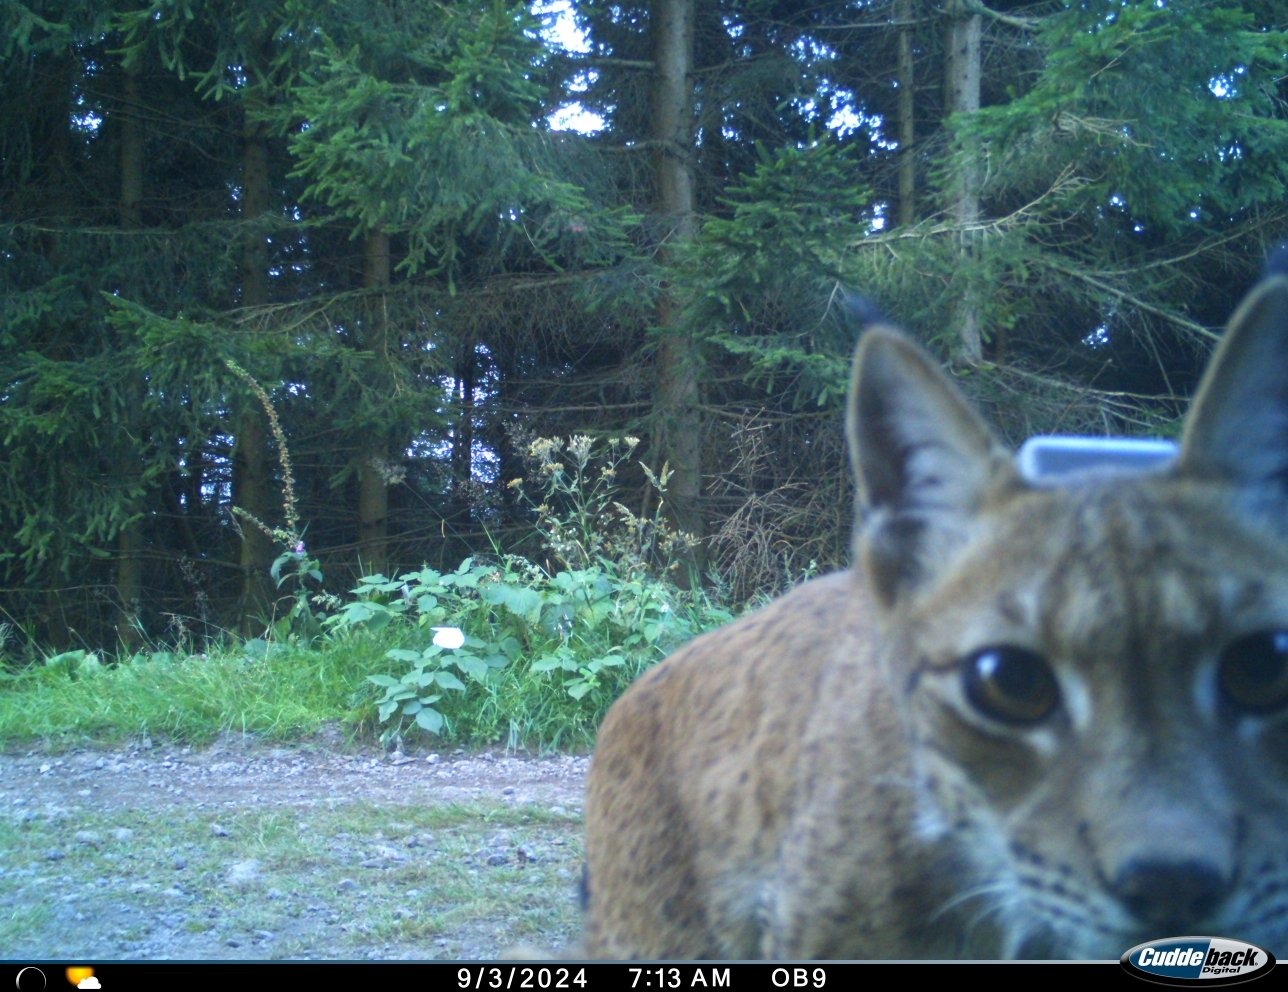
\includegraphics[width = .5\textwidth]{ex_tex/lynx_image}
\end{figure}

\noindent Researchers generate the following counterfactual explanations.

\subsubsection*{Counterfactual I1}

\begin{quote}
	``If the spotted fur pattern were less visible and the nose would be smaller and more pointed, the image would have been classified as a fox.''
\end{quote}

\subsubsection*{Counterfactual I2}

\begin{quote}
	``If the background vegetation were greener and denser, the image would have been classified as a fox.''
\end{quote}

\subsubsection*{Counterfactaul I3}
\begin{quote}
	``If several pixels across the image were modified in a way nearly invisible to humans, the image would have been classified as a deer.''
\end{quote}


\subsubsection*{Counterfactual I4}

\begin{quote}
	``If the timestamp watermark were removed, the image would have been classified as a fox.''
\end{quote}

\paragraph{Discuss in groups}

\begin{enumerate}[label=\arabic*.]
	
	\item Which counterfactual(s) appear(s) biologically plausible?
	
	\item Which counterfactual(s) reflects that our model is not robust?
	
	\item Which counterfactual(s) suggest(s) the model may rely on spurious correlations?
	
	\item What does counterfactual I4 suggest about the dataset or data collection process?
	
	\item Which counterfactual(s) would concern you most as a machine learning engineer?
	
	\item Are any of these counterfactuals actionable? If yes, for whom?

\end{enumerate}

\end{document}